% chap5.tex (Methodology and Result)

\chapter{Methodology and Result}

Traditioanlly, a single type of predictor served to predict the energy demand of all powertype customers. Since each powertype customers acts differently, I have attempted to attack each type of customer separately to make a prediction mechanism that perfroms better than the baseline predictor.

\section{Baseline Predictor}
Baseline predictor is the default prediction mechanism provided by the PowerTAC system. It exploits the fact that usage of a timeslot of a customer in a specific date is highly correlated with the day of the week and the time slot. To make prediction it stores the average energy usage of an hour of a week. So, for each customer it uses $24*7 = 168$ memory to remember average usages. As soon as it learns about a new usage information of an hour of a week, it updates old average using the following algorithm.


\begin{algorithm}
\caption{Calculate average usage for day d and timeslot t, $avgUsage$}
\begin{algorithmic} 
\STATE Initialize
\STATE $avgUsage = 0$
\STATE Update
\STATE $avgUsage = 0.7 * avgUsage + 0.3 * oldUsage$
\STATE Predict usage for day d and time slot t
\STATE return $avgUsage$
\end{algorithmic}
\end{algorithm}

There will be another type of predictor that is designed to make prediction for a single customer. In general, if there are n customers in the system, we will need n predictor each one trained on a single customer. I went further by checking different machine learning algorithms such as M5Tree, Linear Regression, M5P rules and REP tree for each customer and picked the best performing one for each customer.

\section{Prediction Mechanism}

In this section I will describe how I attempted to make predictor for each of the powertypes.

\subsection{Consumption Type Customer}
For the consumption type customers, the following algorithm is used to make prediction about them.
\begin{algorithm}
\caption{Make prediction for consumption type customer}
\begin{algorithmic} 
\STATE Extract features for each time slot for each customer
\STATE Train kmeans cluster for different sizes of k
\STATE pick suitable value for k
\STATE For each cluster out of k clusters, find the best performing predictor.
\STATE train individual classifer for each customer
\STATE evaluate performance using test data
\end{algorithmic}
\end{algorithm}

To make the cluster, the extractor program extracts consumption customer's information from 30 game logs. In the first phase, it collects the weekly usages. So from each log file and for each customer, the program extracts 24 * 7 values, each of the value represent average usage of an hour in a weekday. In the second phase, the clustering algorithm clusters based on the extracted weekly average usages. Once the cluster is made, the second extractor programs extracts slot based information of all the customers in a given slot and makes a training set out of it. In the next phase, a program creates creates several machine learning predictors such as linear regression, decision trees etc and figures out which performs best for the cluster. The best performing predictor is used to make prediction about the cluster. In the runtime, a customer will be grouped in a cluster based on its weekly usage. Once the program knows the cluster assigned for a customer, the program loads the corresponding predictor to predict about the new customer. 

%feature extraction

For the consumption type customers, the following algorithm is used to extract feature
\begin{algorithm}
\caption{extract information from transactionReport sent to broker after each time slot through TariffTransactionHandler call back method}
\begin{algorithmic} 
\STATE timeSlot = get time slot from transactionReport
\STATE customerName = get customer name from transactionReport
\STATE energyUsed = get energy used from trom transactionReport
\STATE addUsage(customerName, timeSlot, energyUsed)
\end{algorithmic}
\end{algorithm}

%write extracted features
For the consumption type customers, the following algorithm is used to write the extracted features after all information is received from a timeslot
\begin{algorithm}
\caption{write extracted data after timeSlot update message received from TimeSlotUpdateHandler call back method}
\begin{algorithmic} 
\STATE knownTimeSlot = timeSlot - 1
\FOR{each customer}
\STATE day = get day of knownTimeSlot
\STATE hour = get hour of knownTimeSlot
\STATE statisticalData = get statistics of the customer of day and hour
\STATE weatherData = get weather data of knownTimeSlot
\STATE trueUsage = get true usage of customer in knownTimeSlot
\STATE trainingInstance = create training instance by combining statisticalData, WeaterData and trueUsage 
\STATE writeToFile(trainingInstance)
\ENDFOR
\end{algorithmic}
\end{algorithm}

%write weekly avg of each customer
For the consumption type customers, the following algorithm is used to write the average usage of each slot of week
\begin{algorithm}
\caption{write average usage of customer of each hour of the week}
\begin{algorithmic} 
\REQUIRE information of all timeslots have been received
\FOR{each customer}
	\STATE trainingInstance = create empty training instance
	\FOR{each day of week}
		\FOR{each hour of day}
			\STATE averageUsage = get average usage of day and hour of customer
			\STATE append averageUsage to the trainingInstance
		\ENDFOR
	\ENDFOR
	\STATE writeToAvgUsageFile(trainingInstance)
\ENDFOR
\end{algorithmic}
\end{algorithm}

%make cluster

\begin{algorithm}
\caption{create kmeans cluster of size k from weekly usage training instance file}
\begin{algorithmic} 
\STATE data = load weekly average usage file
\STATE kmeansCluster = build kmeans cluster of size k
\STATE save kmeansCluster
\end{algorithmic}
\end{algorithm}


%observe error of each cluster

%find size of k
\begin{algorithm}
\caption{find error of kmeans clusters of different size}
\begin{algorithmic} 

\FOR{each cluster size k}
	\STATE get the kMeansCluster of size k
	\FOR{cluster in KMeansCluster}
		\STATE combine slot based training instances of that cluster
		\STATE train linear regression classifier based on the combined data
		\STATE save the classifier for cluster
	\ENDFOR
\ENDFOR

\FOR{each training instance}
	\STATE compute error of the instance using each kMeansCluster
\ENDFOR
\end{algorithmic}
\end{algorithm}

%calculate error
\begin{algorithm}
\caption{calculate error from predictedValue and trueValue}
\begin{algorithmic} 
\STATE absoluteError = abs(predictedValue - trueValue)
\STATE relativeAbsoluteError = (absoluteError / trueValue ) * 100 \%
\end{algorithmic}
\end{algorithm}

%find best classifier for cluster of size k
\begin{algorithm}
\caption{find best classifiers of each cluster of kmeans cluster of size k}
\begin{algorithmic}
\FOR{each cluster in kMeansCluster}
	\STATE combine slot based data of the all the customers in cluster
	\STATE train available classifiers on the combined data using 10 fold cross validation
	\STATE choose the classifier with minimum error
	\STATE save the classifier for making prediction for cluster
\ENDFOR 
\end{algorithmic}
\end{algorithm}

%find best classifier for individual customers
\begin{algorithm}
\caption{find best classifiers created for each individual customer}
\begin{algorithmic}
\FOR{each customer}
	\STATE combine all slot based training instance of the customer
	\STATE train available classifiers on the combined data using 10 fold cross validation
	\STATE choose the classifier with minimum error
	\STATE save the classifier for making prediction about the customer
\ENDFOR 
\end{algorithmic}
\end{algorithm}

%Testing
\begin{algorithm}
\caption{performance evalulation of each method}
\begin{algorithmic}
\FOR{each training instance}
	\STATE classify using moving average usage
	\STATE classify using individual prediction mechanism
	\STATE classify using cluster based predictor
	\STATE find and accumulate errors of each mechanism
\ENDFOR 
\STATE find averageError from the accumulated errors
\end{algorithmic}
\end{algorithm}


\section{Result}
\subsection{Finding number of clusters}

At first, I have segmented the customer using KMeans clustering algorithm with cluster sizes = 4, 5, 6, 7, 8, 9, 10 and 11. For KMeans with size k, we will have k clusters. For each of the k clusters I had a linear regression predictor. I observed the relative percentage error and absolute average the above cluster sizes. Figure \ref{fig:cluster-type-vs-error} shows the result. From, the figure it is clear that the size of the cluster does not have a big impact on the prediction performance.

\begin{figure}[h!]
  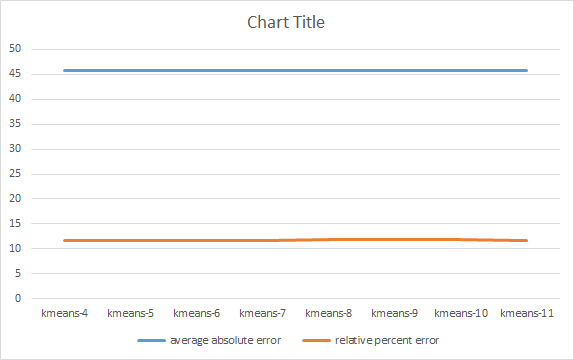
\includegraphics[width=\linewidth]{cluster-types-vs-error.png}
  \caption{Cluster type vs Error.}
  \label{fig:cluster-type-vs-error}
\end{figure}

To keep things simple, I have decided to choose Kmeans cluster of size 4. The figure \ref{fig:4-cluster-with-10-files} shows the assignments of customers in different clusters. From the figure, cluster-0 holds most of the offices, cluster 2 holds most of the village types, cluster 3 holds the medical center, cluster 1 holds large housing such as brooksidehomes, centerville homes etc.

\begin{figure}[h!]
  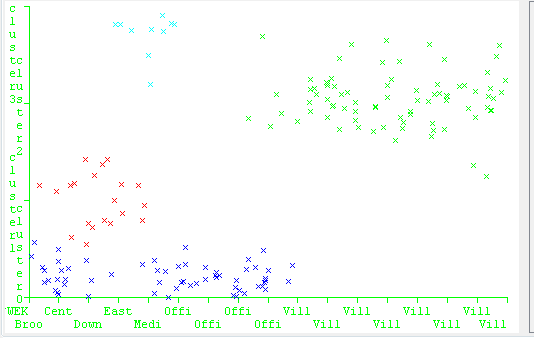
\includegraphics[width=\linewidth]{4-cluster-with-10-files.png}
  \caption{Cluster assignments.}
  \label{fig:4-cluster-with-10-files}
\end{figure}

\subsection {Finding best predictor for each cluster}
I have used the following features for a given timeslot to train prediction models. 
 
\begin{itemize}
  \item Temperature
  \item Cloud Cover
  \item Wind Speed
  \item Average of the Slot
  \item Standard Deviation of the Slot
\end{itemize}

Next, I have tried out  M5Tree, Linear Regression, M5P rules and REP tree machine learning algorithms to see which one performs best for each of the 4 clusters. Figure \ref{fig:cluster-0-predictors}, \ref{fig:cluster-1-predictors}, \ref{fig:cluster-2-predictors}, \ref{fig:cluster-3-predictors} show that M5P, M5P, REPTree and M5RULES are the best predictors for cluster 0, 1, 2 and 3 respectively.


\begin{figure}[h!]
  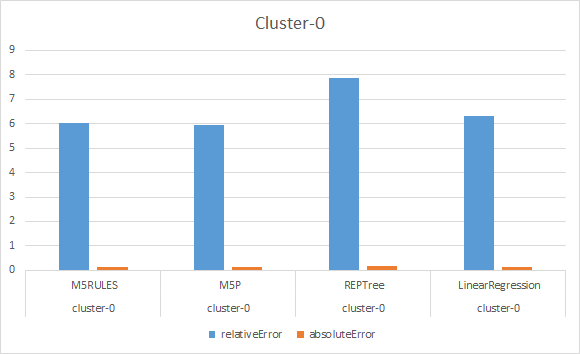
\includegraphics[width=\linewidth]{cluster-0-predictors.png}
  \caption{Performance of differenc predictors for cluster 0}
  \label{fig:cluster-0-predictors}
\end{figure}

\begin{figure}[h!]
  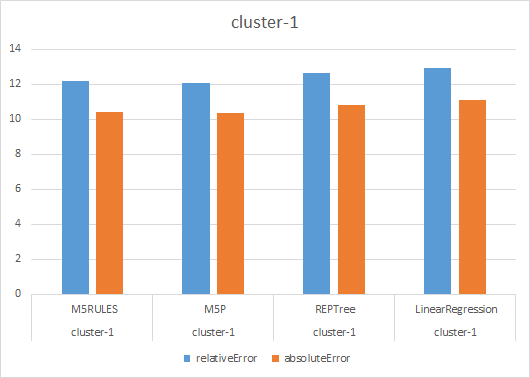
\includegraphics[width=\linewidth]{cluster-1-predictors.png}
  \caption{Performance of differenc predictors for cluster 1}
  \label{fig:cluster-1-predictors}
\end{figure}


\begin{figure}[h!]
  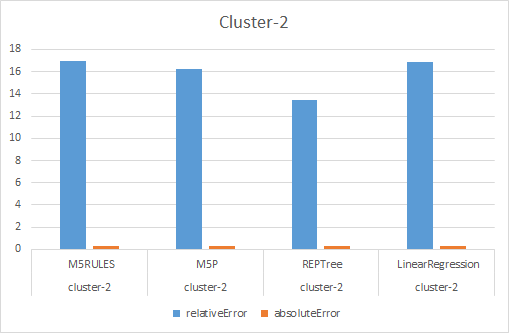
\includegraphics[width=\linewidth]{cluster-2-predictors.png}
  \caption{Performance of differenc predictors for cluster 2}
  \label{fig:cluster-2-predictors}
\end{figure}


\begin{figure}[h!]
  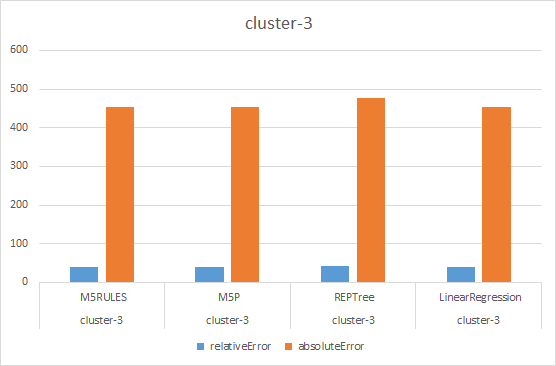
\includegraphics[width=\linewidth]{cluster-3-predictors.png}
  \caption{Performance of differenc predictors for cluster 3}
  \label{fig:cluster-3-predictors}
\end{figure}

The next step is to find the best predictors for each of the customers. Based on the data from each of the customers, the above four types of predictors were tried out. For each customer, the following predictors performed the best. 

\begin{table}[h!]
\centering
\begin{tabular}{|c| c|} 
 \hline
 Customer Name & Best Predictor Type \\ [0.5ex] 
 \hline
BrooksideHomes &	M5P \\
CentervilleHomes &	M5P \\
DowntownOffices &	M5P \\
EastsideOffices &	M5P \\
OfficeComplex 1 NS Base &	LinearRegression \\
OfficeComplex 1 SS Base &	LinearRegression \\
OfficeComplex 2 NS Base &	LinearRegression \\
OfficeComplex 2 SS Base &	LinearRegression \\
Village 1 NS Base &	M5P \\
Village 1 RaS Base &	LinearRegression \\
Village 1 ReS Base &	M5P \\
Village 1 SS Base &	M5P \\
Village 2 NS Base &	LinearRegression \\
Village 2 RaS Base &	M5P \\
Village 2 ReS Base &	M5P \\
Village 2 SS Base &	M5P \\
MedicalCenter@1	& M5P \\ [1ex] 
 \hline
\end{tabular}
\caption{Best individual predictor for each customer}
\label{table:1}
\end{table}

The figure \ref{fig:indiv-cutomer-best-predictor-error} shows error percentage of each of the predictors type for each of the customer types.

\begin{figure}[h!]
  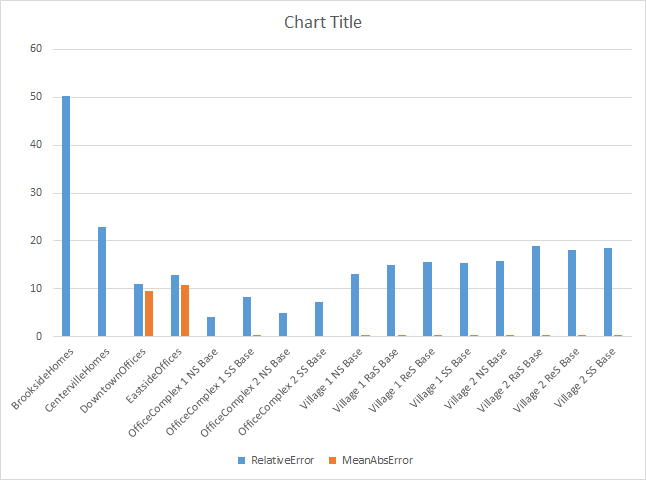
\includegraphics[width=\linewidth]{indiv-cutomer-best-predictor-error.png}
  \caption{Performance of the best predictors for each customer type. Customer Medical center was excluded as it was showing huge error. }
  \label{fig:indiv-cutomer-best-predictor-error}
\end{figure}

Finally, the cluster based prediction and the two baselines were tested with data extracted from 5 test files that were not used for training. From Figure \ref{fig:prediction-scheme-vs-error} we can see that cluster based prediction mechanism performed almost as well as the mechanism where n predictors are needed for n customers. And it did well than the moving average prediction scheme.

\begin{figure}[h!]
  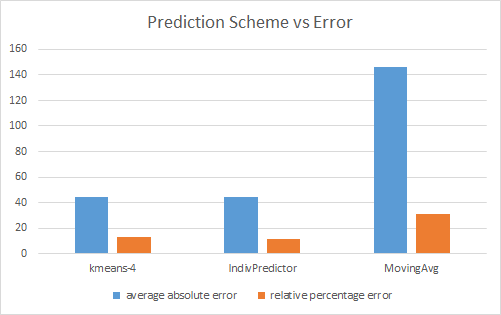
\includegraphics[width=\linewidth]{prediction-scheme-vs-error.png}
  \caption{Performance of the three prediction mechanisms. Cluster based predictor performs as good as the individual predictor for each customers and performs better than the moving average predictor. }
  \label{fig:prediction-scheme-vs-error}
\end{figure}